\documentclass{ieeeaccess}
\usepackage{lineno,hyperref}
\usepackage{graphicx} 
\usepackage{subcaption}
\usepackage{ulem}
\usepackage{booktabs}
\usepackage{algorithm,algpseudocode}
\usepackage{amsmath}
\usepackage{tabularx}
\usepackage[utf8]{inputenc}
\usepackage[english]{babel}
\usepackage[LAE,T1]{fontenc}
\usepackage{bigstrut}
\usepackage{adjustbox} %\bottomrule
\usepackage{multicol, blindtext}
\usepackage{kantlipsum}
\usepackage{makecell}
\usepackage{adjustbox} %
\usepackage{multirow}
\usepackage{rotating}
\usepackage{pdflscape}
\usepackage{epstopdf}
\usepackage{color,soul}
\usepackage{natbib}
\usepackage{enumitem}
\DeclareUnicodeCharacter{00A0}{ }
\DeclareUnicodeCharacter{00A0}{~}
\DeclareUnicodeCharacter{0301}{\'{e}}
\DeclareUnicodeCharacter{2212}{-}
\newcolumntype{H}{>{\iffalse}c<{\fi}@{}}
\usepackage{url}
\usepackage{graphics}
\usepackage{caption}
\usepackage{booktabs,tabularx,dcolumn}
\usepackage{epstopdf}
\usepackage{amsmath,amssymb,amsfonts}
\usepackage{textcomp}
\usepackage[english]{babel}
\usepackage{blindtext}
 
\graphicspath{{./images/}}
\def\BibTeX{{\rm B\kern-.05em{\sc i\kern-.025em b}\kern-.08em
    T\kern-.1667em\lower.7ex\hbox{E}\kern-.125emX}}

\TeXXeTstate=1
\begin{document}
\history{Date of submission Jan, 2024}
\title{An Extractive Video Summarization App Employing NLP Techniques }

\author{\uppercase{Abdelrahman Ayman}, \authorrefmark{1}
\uppercase{Ahmed Sameh}, \authorrefmark{2}
\uppercase{Elsaeed Ahmed}, \authorrefmark{3}
\uppercase{Sohayla Ihab}, \authorrefmark{4}
\uppercase{Tasneem Hisham} \authorrefmark{5}
}
\address[1]{Computer Engineering and Software Systems, Ain Shams University, 19p6458}
\address[2]{Computer Engineering and Software Systems, Ain Shams University, 19p5861}
\address[3]{Computer Engineering and Software Systems, Ain Shams University, 19p1087}
\address[4]{Computer Engineering and Software Systems, Ain Shams University, 19p7343}
\address[5]{Computer Engineering and Software Systems, Ain Shams University, 19p4152}

\begin{abstract}
This paper presents a comprehensive study of Natural Language Processing (NLP) techniques applied to video summarization. Video content is growing rapidly, making it increasingly challenging for users to efficiently consume and navigate through vast amounts of visual information. Video summarization aims to generate concise and representative summaries that capture the key aspects of a video. In recent years, NLP has emerged as a powerful tool to enhance video summarization by leveraging textual information associated with videos, such as titles, descriptions, and subtitles.
\\\\
The objective of this research is to explore various NLP approaches employed for video summarization. At first divide, there are two main approaches to video summarization, abstractive and extractive. 
Abstractive summarization involves generating a summary that may contain new phrases, sentences, or even rephrased information that captures the essence of the original text. Extractive summarization involves selecting and combining the most important sentences or phrases from the source text to create a summary.
\\\\
The study encompasses an analysis of NLP techniques including Pure NLTK, TextRank, LexRank, Text Summing and Naive Reduction. Each of these techniques are encapsulated in corresponding pipelines to tokenize, score, graph or rank words and their frequencies. After that, summaries are generated in order in the form of shortened videos.
\\\\
The results of the evaluation demonstrate the effectiveness and potential of NLP techniques in video summarization regardless of video length, accent or even language. 
The findings highlight the effect of various NLP techniques on the form of the generated summaries. In addition, a comparison with state-of-the-art methodologies is performed to provide clearer insights into the quality of the summaries, not only with regards to application quality but also in regards to existing use cases. The study concludes by discussing the implications of the research findings and application tests. Finally, we propose future directions for video summarization enhancement and personalization.
\end{abstract}

\begin{keywords}
Video Summarization, Extractive Summarization, Text Scoring, Natural Language Processing(NLP), Toolkits
\end{keywords} 
%\titlepgskip=-15pt

\makeatletter
\newcommand{\@doi}{}
\makeatother

\maketitle

\section{Introduction}
\label{introduction}
The proliferation of digital video content has become a defining characteristic of the modern internet era. With an average user consuming over 17 hours of video per week and platforms like YouTube receiving 500 hours of video uploads every minute, the ability to quickly process and understand video content has never been more critical \cite{ref7}. This immense volume of data presents unprecedented challenges in storage, retrieval, and indexing, necessitating sophisticated video summarization solutions to distill vast streams of visual information into accessible and manageable forms.

Recent advancements in video summarization have evolved from manual annotation to automated techniques that leverage the advancements in artificial intelligence, particularly in natural language processing (NLP) and machine learning (ML) \cite{DNN5}. The transformative potential of deep learning has been demonstrated in its ability to create concise, representative summaries by intelligently selecting key frames and sequences \cite{duc}. This progression towards automation has facilitated the handling of large-scale video data, allowing for summarization that is not only rapid but also contextually relevant and personalized \cite{ref2}.

The challenge of catering to specific user needs and contextual relevance in video summaries remains at the forefront of the field. Addressing this, we draw inspiration from the advanced methodologies and diverse perspectives on video summarization outlined in the related work, such as the machine learning procedures that analyze statistical and computer vision methods, as well as the deep learning techniques that utilize neural networks \cite{Lexrank}. Moreover, the personalized and query-relevant summarization techniques highlighted by key contributions from recent research underscore the complexity and necessity for adaptable algorithms \cite{ref5}.

Our research aims to bridge the gap between the current state-of-the-art and the practical requirements of video summarization by introducing a comprehensive suite of NLP techniques. We present an innovative extractive video summarization application that employs a curated selection of NLP algorithms, including the Pure NLTK Method, Gensim TextRank, Luhn's Heuristic, LexRank, KL-Sum, and Naïve Reduction Method \cite{ref6}. Our approach emphasizes the importance of algorithmic diversity and user-friendliness, providing a functional and intuitive tool for end-users \cite{ref2}.

This paper details our development process, highlighting the integration of various summarization algorithms and the iterative refinements that led to an application excelling in both performance and user experience \cite{ref1}. We present a user-friendly interface designed through an iterative process involving user feedback, thereby ensuring that our application is not only powerful but also accessible \cite{ref8}.

In summary, we contribute a significant step towards realizing the full potential of video summarization, offering a scalable and effective solution that benefits various domains where quick and accurate video analysis is essential \cite{ref5}. The following sections will delve into our development approach, algorithm selection, implementation details, and the practical implications of our work.


\section{related work}
\label{related_work}
The field of video summarization and processing has witnessed significant advancements, with various innovative methodologies and applications. This section comprehensively explores key contributions from recent research papers, bringing together diverse perspectives on video summarization.

\subsection{Machine Learning Procedures}
These procedures can depend on statistical, analytic or computer vision methods. Datasets found to be used here are either collections of documents, video links or json segmented video transcripts\cite{duc}\cite{summe}.
\begin{itemize}
  \item \textbf{Hidden Markov Model: } This statistical model assumes the relationship between probability densities of different words in a labelled json segmented dataset. This is done by transition probabilities of unsummarized json fields and emission probabilities of the expected keywords. The output of this model is a transcript summary of the video.
  \item \textbf{Shot Segmentation Model: } This model\cite{ML1} uses computer vision to segment a local video dataset utilizing features such as histogram and pixel differences. They also introduce Independent Component Analysis (ICA) to extract features for describing the content of a shot. This model works with unlabelled local video datasets. The aim is to generate critical windows.
  Hierarchical clustering of these windows provides a summarization of the shots, preserving the original component objects that make up the video and characterizing the semantically essential information present in the video.
  The advantage of this technique over other keyframe-based approaches is the preservation of original component objects and the generation of automatic textual annotations for video shots. The output of this model is a summarized video. 
  \item \textbf{Other statistical models: } Examples of those include Naive Bayes, Decision Trees and Random Forest.
\end{itemize}

\begin{figure}	[!htb]
    \centering
    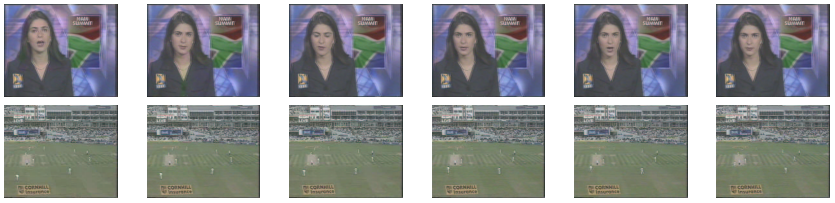
\includegraphics[width=8cm, height=9cm, keepaspectratio]{images/ShotsICA.PNG}
    \caption{Critical window extraction example of a news report and a sports match}
    \label{shots_example}
\end{figure}

    
\subsection{Deep Learning Procedures: }
These procedures are usually ones that involve neural network models. Datasets found to be used here are labelled video transcript datasets.\cite{DNN1}
\begin{itemize}
    \item \textbf{General Model: } This is a simple realization of the model that involves an Encoder with an Embedding input followed by an LSTM(Long Short Term Memory) hidden layer\cite{DNN4}. The hidden layer produces a fixed-length representation of the source documents. The decoder reads the representation along with the Embedding of the last generated word and uses these inputs to generate each word in the output.
    \item \textbf{One-Shot Model: } This model generates an entire output sequence in a single shot. In this model, the decoder solely uses the context vector to generate the output sequence.
    \item \textbf{Recursive Models: }This model\cite{DNN7} is a recursive implementation of the Encoder-Decoder architecture. It involves feeding the output of the decoder back into the input of the decoder recursively until the end of the sequence is reached. Another variant of this model is one that involves feeding the output of the decoder back into the input of the encoder recursively until the end of the sequence is reached.
\end{itemize}
    
\subsection{Natural Language Processing Procedures} 
These procedures are best at improving user experience in many ways:
\begin{itemize}
     \item \textbf{Summarization: } NLP algorithms can be used to summarize video, audio, and textual content, providing users with concise and informative summaries.
    
     \item \textbf{Speech Recognition: } NLP-based speech recognition technology can transcribe audio content into text, making it searchable and accessible. This capability enhances the user experience by enabling users to interact with and navigate audio content more effectively .
    
     \item \textbf{Text Analysis: } NLP techniques can analyze textual content associated with multimedia, such as comments, descriptions, and transcripts, to extract valuable insights and sentiments.
    
     \item \textbf{Video Summarization in Python NLP Toolkits: \cite{IBM-Watson} }
     There are two different summarization techniques, abstractive and extractive. Abstractive techniques involve creating new sentences from scoring word importance. Extractive techniques involve only using existing sentences and words to compose a summary. The libraries used include Gensim, NLTK, Spacy, and Sumy. The dataset that can be used here is pretty flexible, json, csv transcripts and videos. The results conclude that NLP models work well with a variety of data and are easily embedded in front end frameworks and user friendly apps\cite{ML2}\cite{NLP2}.
\end{itemize}

\begin{figure}	[!htb]
\centering
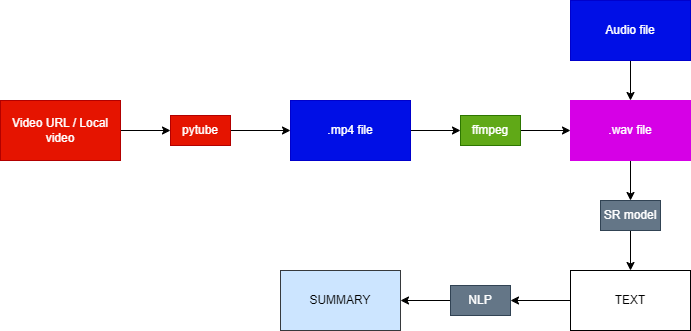
\includegraphics[width=8cm, height=9cm, keepaspectratio]{images/NLP_Arch.png}
\caption{Video Summarizer Sample in NLP techniques}
\label{video_summarizer_example}
\end{figure}

\subsection{Advanced Summarization Techniques}
\begin{itemize}
    \item \cite{ref1} introduces a sequential decision-making process in video summarization using a Deep Summarization Network (DSN), employing reinforcement learning for generating concise and representative summaries.
    \item The research in \cite{ref2} proposes a soft self-attention mechanism for supervised keyshots-based video summarization, improving computational efficiency and setting new performance benchmarks.
    \item In \cite{ref3}, a novel technique for summarizing diverse Internet videos is presented, enhancing standard methods through the use of deep video features encoding content semantics.
\end{itemize}

\subsection{Personalized and Query-Relevant Summarization}
\begin{itemize}
    \item \cite{ref7} explores query-relevant video summarization, utilizing textual-visual semantic embeddings to create summaries that are diverse, representative, and relevant to specific textual queries.
    \item The study in \cite{ref9} addresses summarizing videos recorded by dynamic, independently operating cameras. It presents a framework for identifying important events and selecting the most representative views, contributing a new multi-view egocentric dataset, Multi-Ego.
\end{itemize}

\subsection{Efficient Data Selection and Processing}
\begin{itemize}
    \item The iterative projection and matching algorithm introduced in \cite{ref4} offers a breakthrough in data selection for computer vision tasks, including video summarization.
    \item \cite{ref5} examines Video-Language Pretraining (VLP) from an egocentric perspective, providing insights into video-text relationships in this specific domain.
    \item \cite{ref6} proposes a comprehensive approach to video understanding, treating videos as sequences of clips with transferable semantics for various analytical tasks.
    \item FastForwardNet (FFNet), introduced in \cite{ref8}, innovates in video processing by selectively fast-forwarding through content using reinforcement learning.
\end{itemize}

\subsection{Specialized Applications in Video Summarization}
\begin{itemize}
    \item Paper \cite{ref10} develops a system for generating video summaries from seniors' indoor-activity videos captured by a social robot. This research is pivotal in addressing the challenges posed by long video sequences and redundant information in indoor environments.
\end{itemize}

\subsection{Our Contribution}
Our application seamlessly integrates local videos into a user-friendly interface, providing a suite of tools for efficient video summarization. Users begin by selecting one of six summarization methods: Pure NLTK, Gensim, Luhn, LexRank, KL-Sum, or Naive Reduction. Following method selection, users input the compression ratio and upload the video.
\\\\The transcription phase involves an automated library extracting the audio stream, which is then sent to an online API for transcription. Upon receiving the transcription response, it undergoes processing, followed by the application of summarization algorithms to the transcribed content, finally the Original Transcription, Summarized Text and Summarized Video are returned to the User.


\section{Methodology}
In the landscape of information consumption, video summarization emerges as a pivotal tool for enhancing accessibility to extensive content. Our commitment to developing an extractive video summarization app underscores the importance of preserving the essence of the original text. Employing a spectrum of algorithms, our objective is to distill key information while maintaining fidelity to the source material.

\subsection{Algorithms Selection}
Our curated selection of algorithms brings a multifaceted approach to video summarization, leveraging their distinct strengths\cite{textsummarization}.

\subsubsection{Pure NLTK Method for Text Summarization}
The NLTK (Natural Language Toolkit) based text summarization algorithm employs a straightforward approach using basic natural language processing techniques. The goal is to create a summary by assigning importance scores to sentences based on the frequency of non-stop words. This method is implemented using the NLTK library, which provides tools for working with human language data.\\\\
\textbf{Algorithm Overview}
\begin{enumerate}
    \item \textbf{Tokenization and Stop word Removal:}
    \begin{itemize}
        \item The input text is tokenized into words using NLTK's word tokenizer function.
        \item Stop words (common words like "the," "and" etc.) are removed from the tokenized words.
    \end{itemize}
    
    \item \textbf{Word Frequency Calculation:}
    \begin{itemize}
        \item A frequency table is created to count the occurrences of each non-stop word in the tokenized list.
        \item The frequency table is case-insensitive.
    \end{itemize}
    
    \item \textbf{Sentence Tokenization:}
    \begin{itemize}
        \item The input text is tokenized into sentences using NLTK's sentence tokenizer function.
    \end{itemize}
    
    \item \textbf{Scoring Sentences:}
    \begin{itemize}
        \item Each sentence is assigned a score based on the sum of frequencies of words present in that sentence.
        \item The score is determined by checking the frequency of each non-stop word in the sentence and adding them up.
    \end{itemize}
    
    \item \textbf{Calculating Average Score:}
    \begin{itemize}
        \item The average score of all sentences is calculated.
    \end{itemize}
    
    \item \textbf{Generating Summary:}
    \begin{itemize}
        \item Sentences whose scores are higher than a certain threshold (1.2 times the average score) are selected for the summary.
        \item The selected sentences are concatenated to form the final summary.
    \end{itemize}
\end{enumerate}

\subsubsection{Gensim TextRank Method for Text Summarization}
TextRank is a graph-based ranking model designed for summarizing text through a process that involves identifying and ranking important elements within the text. The underlying idea is to represent the text as a graph, where each unit (such as words, phrases, or sentences) is a vertex, and connections between units are represented by edges. The model relies on the collective knowledge of the entire text rather than focusing solely on local information.\cite{textrank}\\\\
\textbf{Algorithm Overview}
\begin{enumerate}
    \item \textbf{Graph Construction:}
    \begin{itemize}
        \item \textbf{Vertices:} Think of each word or sentence in the text as a point (vertex) on a graph.
        \item \textbf{Edges:} Imagine lines connecting related words or sentences. If two words often appear together or two sentences are similar, there's a connection (edge) between them.
    \end{itemize}
    
    \item \textbf{Graph Representation:}
    \begin{itemize}
        \item Picture the graph with all these connected points. Some words or sentences are directly connected, while others are indirectly connected through a chain of connections.
    \end{itemize}
    
    \item \textbf{Initial Scores:}
    \begin{itemize}
        \item Give each word or sentence a starting score. This is like saying, "Okay, at the beginning, every word or sentence has some level of importance."
    \end{itemize}
    
    \item \textbf{Iterative Ranking:}
    \begin{itemize}
        \item Now, let's start improving the scores. The algorithm goes through rounds of checking how important each word or sentence is based on its connections.
        \item If a word is connected to many important words, it becomes more important itself. It's like saying, "If important words like you, then you must be important too."
        \item TextRank uses a damping factor, a number usually set to 0.85. This factor prevents extreme swings in importance scores.
    \end{itemize}
    
    \item \textbf{Convergence:}
    \begin{itemize}
        \item Keep doing this process over and over until things stop changing much. It's like refining the importance scores until they settle down and stay mostly the same.
    \end{itemize}
    
    \item \textbf{Ranking and Selection:}
    \begin{itemize}
        \item Now that we have our final scores, we rank the words or sentences from the most important to the least important.
        \item We pick the top-ranked words or sentences because they are the ones that the algorithm thinks are the most important for summarizing the text.
    \end{itemize}
\end{enumerate}

\subsubsection{Luhn's Heuristic Method for Text Summarization}
Luhn's Heuristic Method is an early approach to text summarization. It suggests that the importance of a word in a document is determined by its frequency. The key idea is to focus on sentences with the highest occurrences of important words (stop words) while avoiding sentences with low occurrences.\cite{textsummarization}\\\\
\textbf{Algorithm Overview}\cite{luhn}
\begin{enumerate}
    \item \textbf{TF-IDF Representation:}
    \begin{itemize}
        \item The algorithm uses a TF-IDF (Term Frequency-Inverse Document Frequency) representation to assign weights to words based on their frequency in the document.
    \end{itemize}
    
    \item \textbf{Word Significance Criteria:}
    \begin{itemize}
        \item Stop words are removed, and stemming (reducing words to their base or root form, like changing "likes" to "like") is applied.
    \end{itemize}
    
    \item \textbf{Sentence Scoring:}
    \begin{itemize}
        \item Sentences are scored based on the concentration of significant content terms.
        \item The score is calculated by considering the number of significant words in a sentence and dividing it by the span (number of words between the first and last significant word).
    \end{itemize}

    \begin{figure}	[!htb]
    \centering
    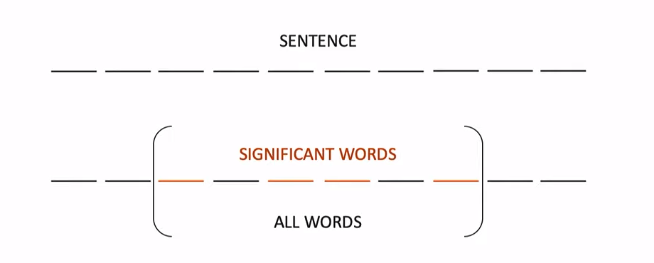
\includegraphics[width=9cm, height=10cm, keepaspectratio]{Luhn.png}
    \caption{Significant Word Example}
    \label{luhn_example}
    \end{figure} 
    
    \item \textbf{Ordering Sentences:}
    \begin{itemize}
        \item Sentences are ordered based on their scores.
        \item The method follows the order in the source documents, meaning sentences are ordered according to their positions in the original text.
    \end{itemize}
\end{enumerate}

\subsubsection{LexRank Method for Text Summarization}
LexRank is a graph-based method for automatic text summarization, akin to PageRank and TextRank. It prioritizes sentences based on their importance using eigenvector centrality in a graph representation.\cite{Lexrank}\\\\
\textbf{Key Concepts}
\begin{itemize}
    \item \textbf{Eigen Vector Centrality and LexRank:}
    \begin{itemize}
        \item Eigen vector centrality calculates the importance of each sentence.
        \item The centrality of a sentence depends on its similarity to other sentences in the document.
    \end{itemize}
    
    \item \textbf{Degree Centrality:}
    \begin{itemize}
        \item Degree centrality is a measure of the importance of a node in a graph based on the number of connections it has (degree).
    \end{itemize}
    
    \item \textbf{TF-IDF (Term Frequency-Inverse Document Frequency):}
    \begin{itemize}
        \item TF-IDF is a numerical statistic that reflects how important a word is to a document in a collection or corpus.
    \end{itemize}
    
    \item \textbf{Power Iteration:}
    \begin{itemize}
        \item Power iteration is an iterative method used to find the dominant eigenvector of a matrix.
    \end{itemize}
\end{itemize}
\textbf{Algorithm Overview}\cite{lexrank2}
\begin{enumerate}
    \item \textbf{Computing Cosine Similarity:}
    \begin{itemize}
        \item Convert Sentences into Vectors using bag-of-words.
        \item Calculate similarity on vectors considering word occurrences.
    \end{itemize}

    \begin{figure}	[!htb]
    \centering
    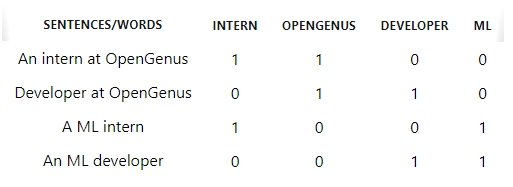
\includegraphics[width=9cm, height=10cm, keepaspectratio]{bagofwords.png}
    \caption{Bag of Words Example}
    \label{bag_of_words}
    \end{figure} 
    
    \item \textbf{Graph Construction:}
    \begin{itemize}
        \item Sentences are the vertices, connection between them is determined by cosine similarity. Nodes having a lot of connections become key sentences (Centroid).
    \end{itemize}

    \begin{figure}	[!htb]
    \centering
    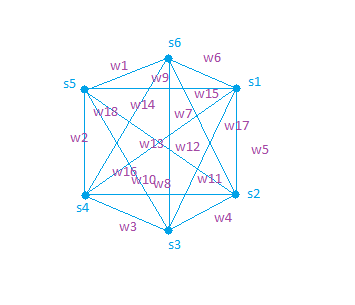
\includegraphics[width=9cm, height=7cm, keepaspectratio]{Lex.png}
    \caption{LexRank Graph Example}
    \label{lexrank_graph}
    \end{figure} 
    
    \item \textbf{Initialization:}
    \begin{itemize}
        \item Initialize arrays for sentences, cosine matrix, degree, LexRank scores, etc.
    \end{itemize}
    
    \item \textbf{Cosine Matrix:}
    \begin{itemize}
        \item Get TF-IDF values, which are numerical statistics that reflect how important a word is to a document in a collection or corpus.
        \item Calculate cosine matrix based on TF-IDF modified values.
        \item Elements greater than a threshold set to 1, others to 0.
    \end{itemize}
    
    \item \textbf{Degree Centrality:}
    \begin{itemize}
        \item Calculate the degree centrality of each sentence.
        \item This determines the importance of each sentence to prevent unrelated sentences from dominating.
    \end{itemize}
    
    \item \textbf{Normalization:}
    \begin{itemize}
        \item Normalize the cosine matrix by dividing each element by the degree of its corresponding node.
    \end{itemize}
    
    \item \textbf{Power Iteration:}
    \begin{itemize}
        \item Use power iteration method to calculate final LexRank scores.
    \end{itemize}
\end{enumerate}

\subsubsection{KL-Sum Method for Text Summarization}
The K-L Sum algorithm, short for Kullback-Leibler Sum algorithm, is a method used for text summarization. The main goal of K-L Sum is to create a summary that is both concise and maintains similarity with the original document in terms of word distribution.\cite{klsum}\\\\
\textbf{Key Concepts}
\begin{itemize}
    \item \textbf{KL Divergence:} This is a measure of how one probability distribution is different from another. In our case, it helps us compute the difference in word distribution between the summary and the source document.
    \item \textbf{Unigram Distribution:} A unigram refers to a single word or token. Unigram distribution represents the frequency or probability distribution of individual words in each sample of text.
    \item \textbf{Connection to Algorithm:} KL Sum algorithm utilizes the KL Divergence to measure the difference between the unigram distribution of the source document and the approximating distribution of the summary. By minimizing this divergence, the algorithm aims to create a summary with a unigram distribution that closely matches that of the original document.
\end{itemize}
\textbf{Algorithm Overview}\cite{kl}  

\begin{figure}	[!htb]
    \centering
    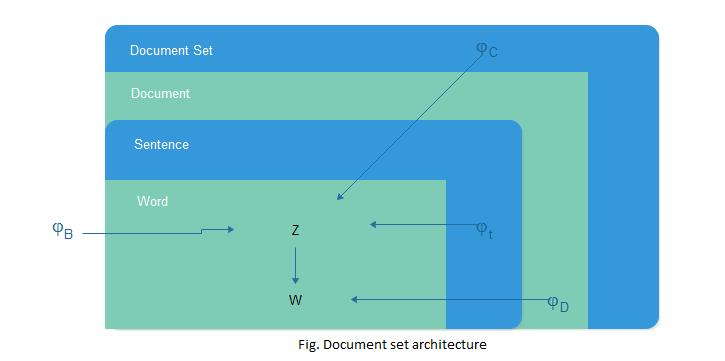
\includegraphics[width=9cm, height=10cm, keepaspectratio]{KL arch.png}
    \caption{KL-Sum Document Architecture}
    \label{klsum_arch}
\end{figure} 

\begin{enumerate}
    \item \textbf{Initialization:}
    \begin{itemize}
        \item Start with an empty set for the summary (S).
    \end{itemize}
    
    \item \textbf{Greedy Optimization:}
    \begin{itemize}
        \item While the length of the summary set is less than or equal to a fixed target length (L):
        \item Iterate through all sentences in the document.
        \item For Each Sentence Compute the KL Divergence (di) between it and the document.
        \item Add the sentence to the summary set if it minimizes Divergence and continue until the target length is reached.
    \end{itemize}
    
    \item \textbf{Ordering Sentences:}
    \begin{itemize}
        \item Order the selected sentences based on their position index (pi) in the source document. This maintains the original order.
    \end{itemize}
\end{enumerate}

\subsubsection{Naïve Reduction Method for Text Summarization}
A graph-based approach for text summarization where we rank sentences or words based on a graph. The focus is to obtain the most important sentences from a single document. Basically, we determine the importance of a vertex within a graph.\\\\
\textbf{Algorithm Overview}\cite{reduction}
\begin{enumerate}
    \item \textbf{Initialization:}
    \begin{itemize}
        \item The algorithm starts by initializing with a set of stop words, common words often excluded from text analysis.
    \end{itemize}
    
    \item \textbf{Sentence Processing:}
    \begin{itemize}
        \item Each sentence in the document is processed to create a set of words, excluding stop words and applying stemming.
    \end{itemize}
    
    \item \textbf{Sentence Rating:}
    \begin{itemize}
        \item The algorithm rates each sentence based on its similarity to other sentences in the document.
        \item Similarity is determined by counting the number of common words between sentences.
    \end{itemize}
    
    \item \textbf{Weight Calculation:}
    \begin{itemize}
        \item For each pair of sentences, the algorithm calculates a weight (rank) by counting common words and normalizing the count.
        \item Normalization involves dividing the count of common words by the logarithm of the product of sentence lengths.
    \end{itemize}

    \begin{figure}	[!htb]
    \centering
    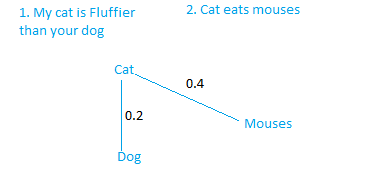
\includegraphics[width=9cm, height=10cm, keepaspectratio]{reduction.png}
    \caption{Reduction Method Weight Calculation Example}
    \label{reduction_example}
    \end{figure} 
    
    \item \textbf{Weight Aggregation:}
    \begin{itemize}
        \item The final weight for a sentence is computed by summing the weights obtained from its similarity to all other sentences.
    \end{itemize}
    
    \item \textbf{Summary Extraction:}
    \begin{itemize}
        \item Sentences with the highest weights are selected for inclusion in the summary.
    \end{itemize}
\end{enumerate}

\subsection{Development Process}
Our developmental journey seamlessly integrated these algorithms, allowing their synergies to augment the summarization capabilities of our app. Iterative refinements were instrumental in addressing challenges, resulting in an application that excels in both performance and user experience.

\begin{figure}	[!htb]
    \centering
    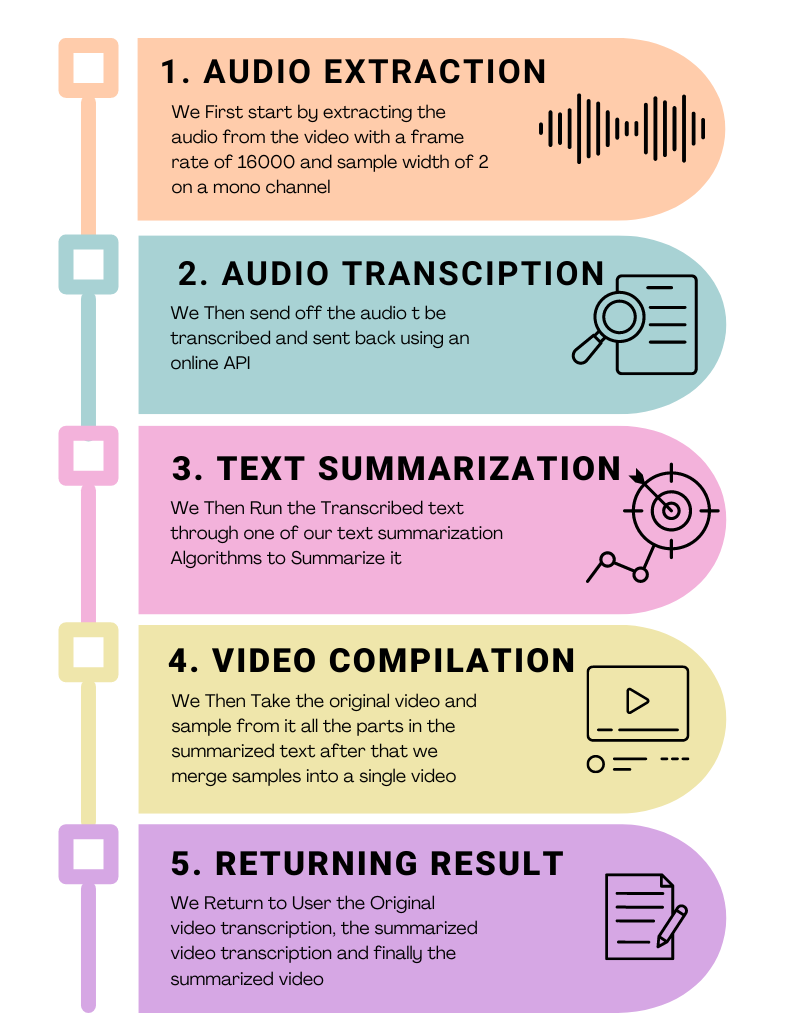
\includegraphics[width=9cm, height=10cm, keepaspectratio]{images/Methodology.png}
    \caption{Development Timeline}
    \label{frameworks_and_libraries}
\end{figure} 

\subsection{Key Principles}
At the heart of our approach lies the key principle of favoring extractive summarization, driven by the overarching goal of preserving the original text. This strategic choice ensures that users receive summarized content that faithfully encapsulates the essence and context of the source material.

\subsection{Project Goals}
Our primary goal is not only to achieve satisfactory summarization results but to pioneer a user-centric paradigm. The design of a simple, intuitive Graphical User Interface (GUI) ensures that users effortlessly engage with the app, transforming the summarization process into a seamless and enjoyable experience.

\subsection{User Interface Design}
Dedicated efforts were channeled into crafting a GUI that prioritizes simplicity and user-friendliness. An iterative process involving user experience testing and feedback loops has culminated in an interface that not only complements the app's functionality but elevates the overall user engagement.

\section{Implementation}
\label{Implementation}
\subsection{Programming Languages and Frameworks}

Our implementation is predominantly built in Python, chosen for its versatility and extensive libraries.

\begin{itemize}
    \item \textbf{Gensim:} Employed the TextRank Summarizer algorithm for robust text analysis and summarization.
    \item \textbf{Sumy:} Utilized for KL-Sum, LexRank, Luhn, and Naive Reduction Text Summarizers, adding diversity to the summarization techniques.
    \item \textbf{json:} Played a key role in parsing Whisper responses, facilitating seamless integration with the speech-to-text functionality.
    \item \textbf{pyqt5:} Implemented the GUI, designed for simplicity and user-friendliness, ensuring an intuitive user experience.
    \item \textbf{nltk:} Utilized for word and sentence tokenization, enhancing text processing capabilities.
    \item \textbf{whisper:} Applied for Speech to Text functionality, providing accurate transcriptions for further analysis.
    \item \textbf{pydub:} Used to extract audio from videos, an essential step in incorporating audio content into the summarization process.
    \item \textbf{moviepy:} Employed for video creation and splitting, enabling efficient handling of video content.
\end{itemize}

\begin{figure}	[!htb]
    \centering
    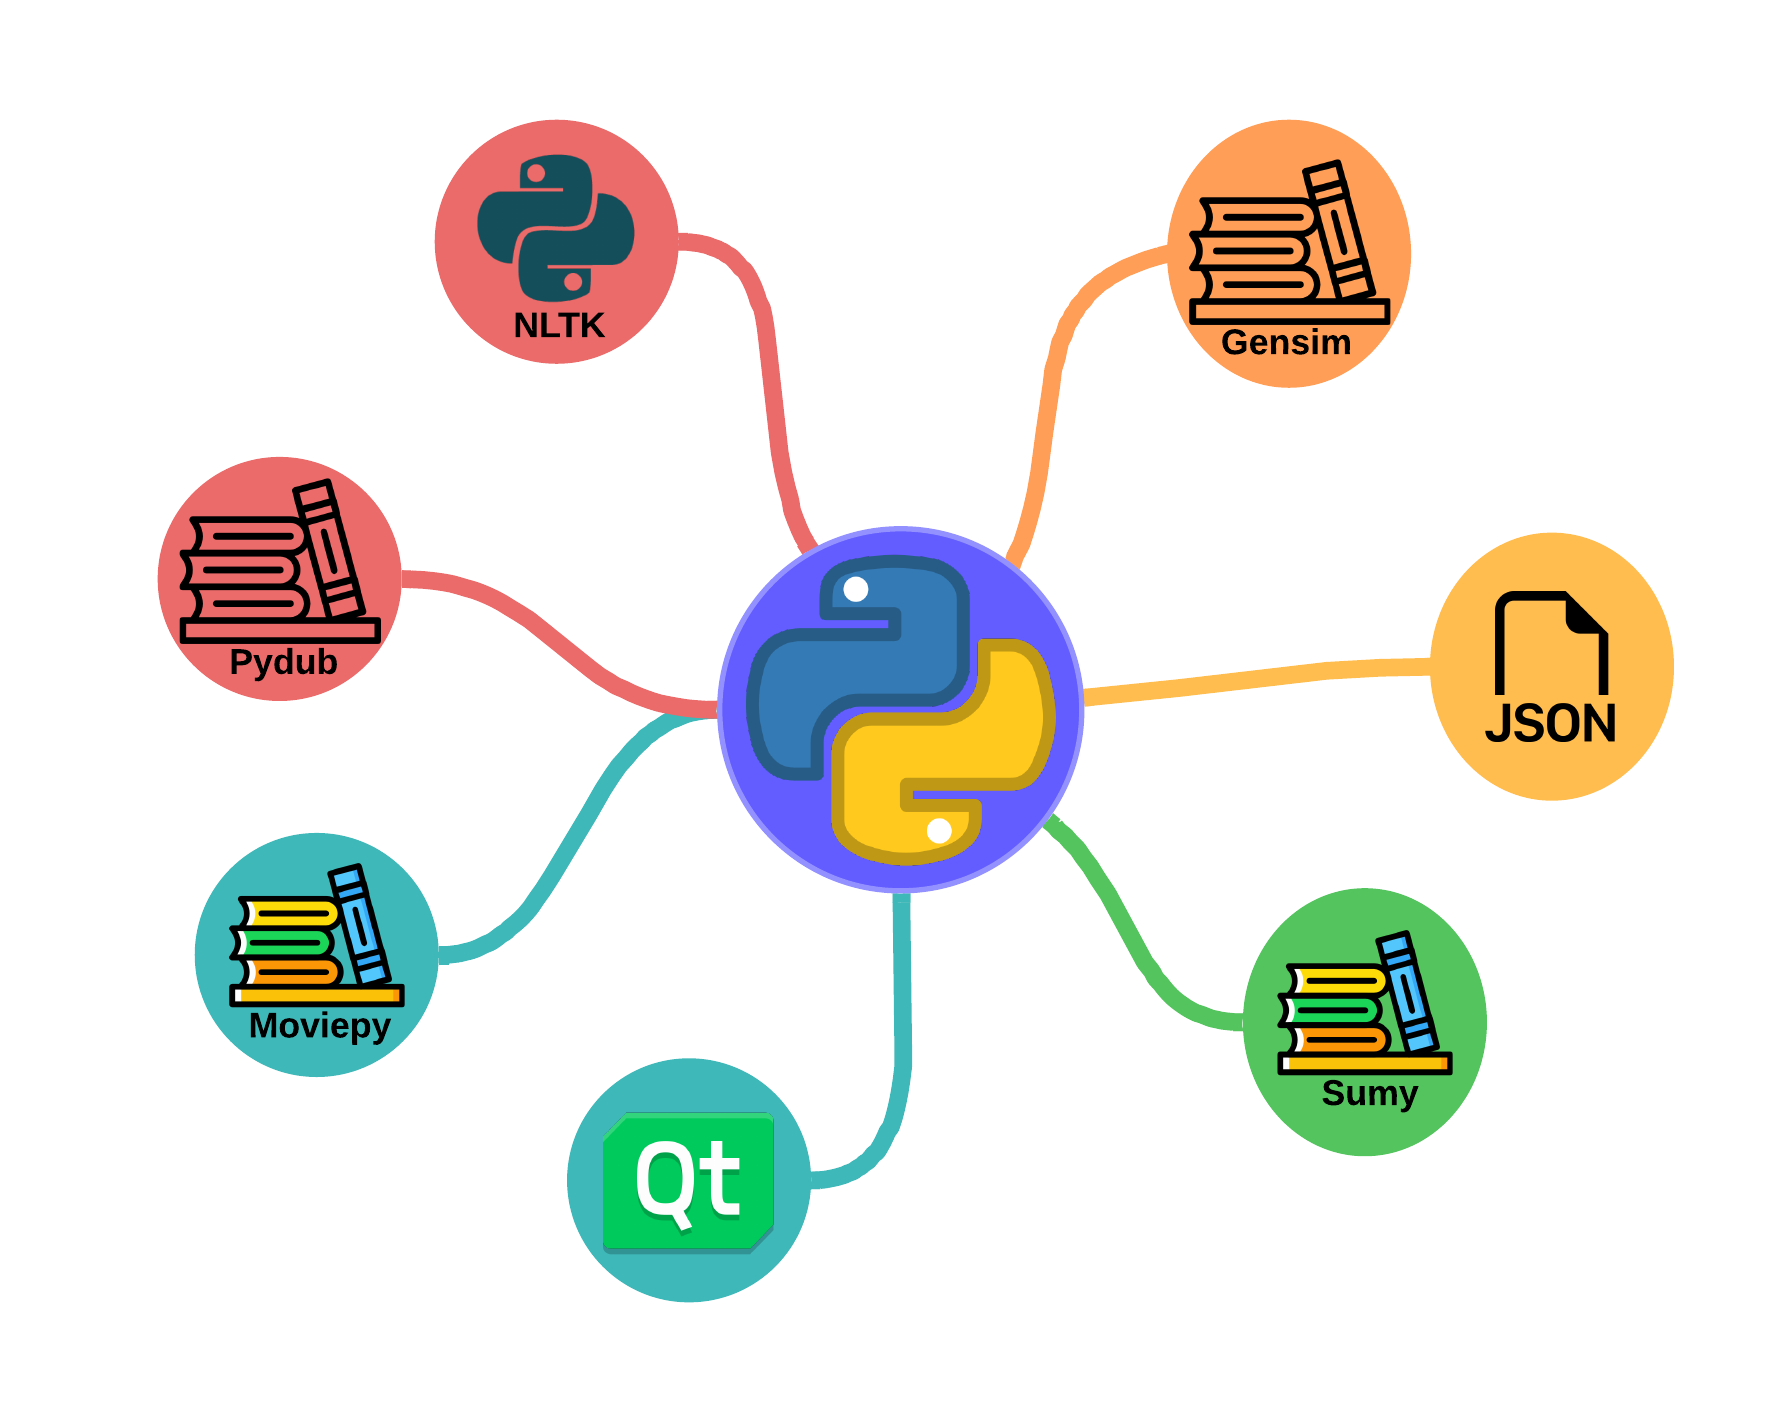
\includegraphics[width=9cm, height=10cm, keepaspectratio]{DevelopmentLibraries.png}
    \caption{Frameworks and Libraries}
    \label{frameworks_and_libraries}
\end{figure} 

\subsection{Data Processing and Integration}

\begin{itemize}
    \item {Audio extraction from videos was meticulously performed using pydub with a frame rate of 16000 and sample width of 2 on a mono channel, ensuring high-quality audio data.}
    \item {Transcription of audio was achieved using the Whisper base model for Speech to Text, allowing for accurate and reliable conversion of spoken words into text.}
    \item {The resulting transcriptions were parsed into JSON format using the json library, facilitating structured data storage and retrieval.}
\end{itemize}

\subsection{Algorithm Integration}

\begin{itemize}
    \item {The Gensim library facilitated the integration of the TextRank Summarizer algorithm, providing a powerful tool for extractive summarization.}
    \item {For KL-Sum, LexRank, Luhn, and Naive Reduction Text Summarizers, the Sumy library was instrumental, enabling a diverse set of algorithms for comprehensive summarization.}
\end{itemize}

\subsection{User Interface Design}

\begin{itemize}
    \item {The GUI, developed using pyqt5, was meticulously crafted for simplicity and user-friendliness.}
    \item {Design principles emphasized a straightforward interface, avoiding complex visuals and overcrowded elements to enhance user understanding and interaction.}
\end{itemize}

\begin{figure}
    \centering
    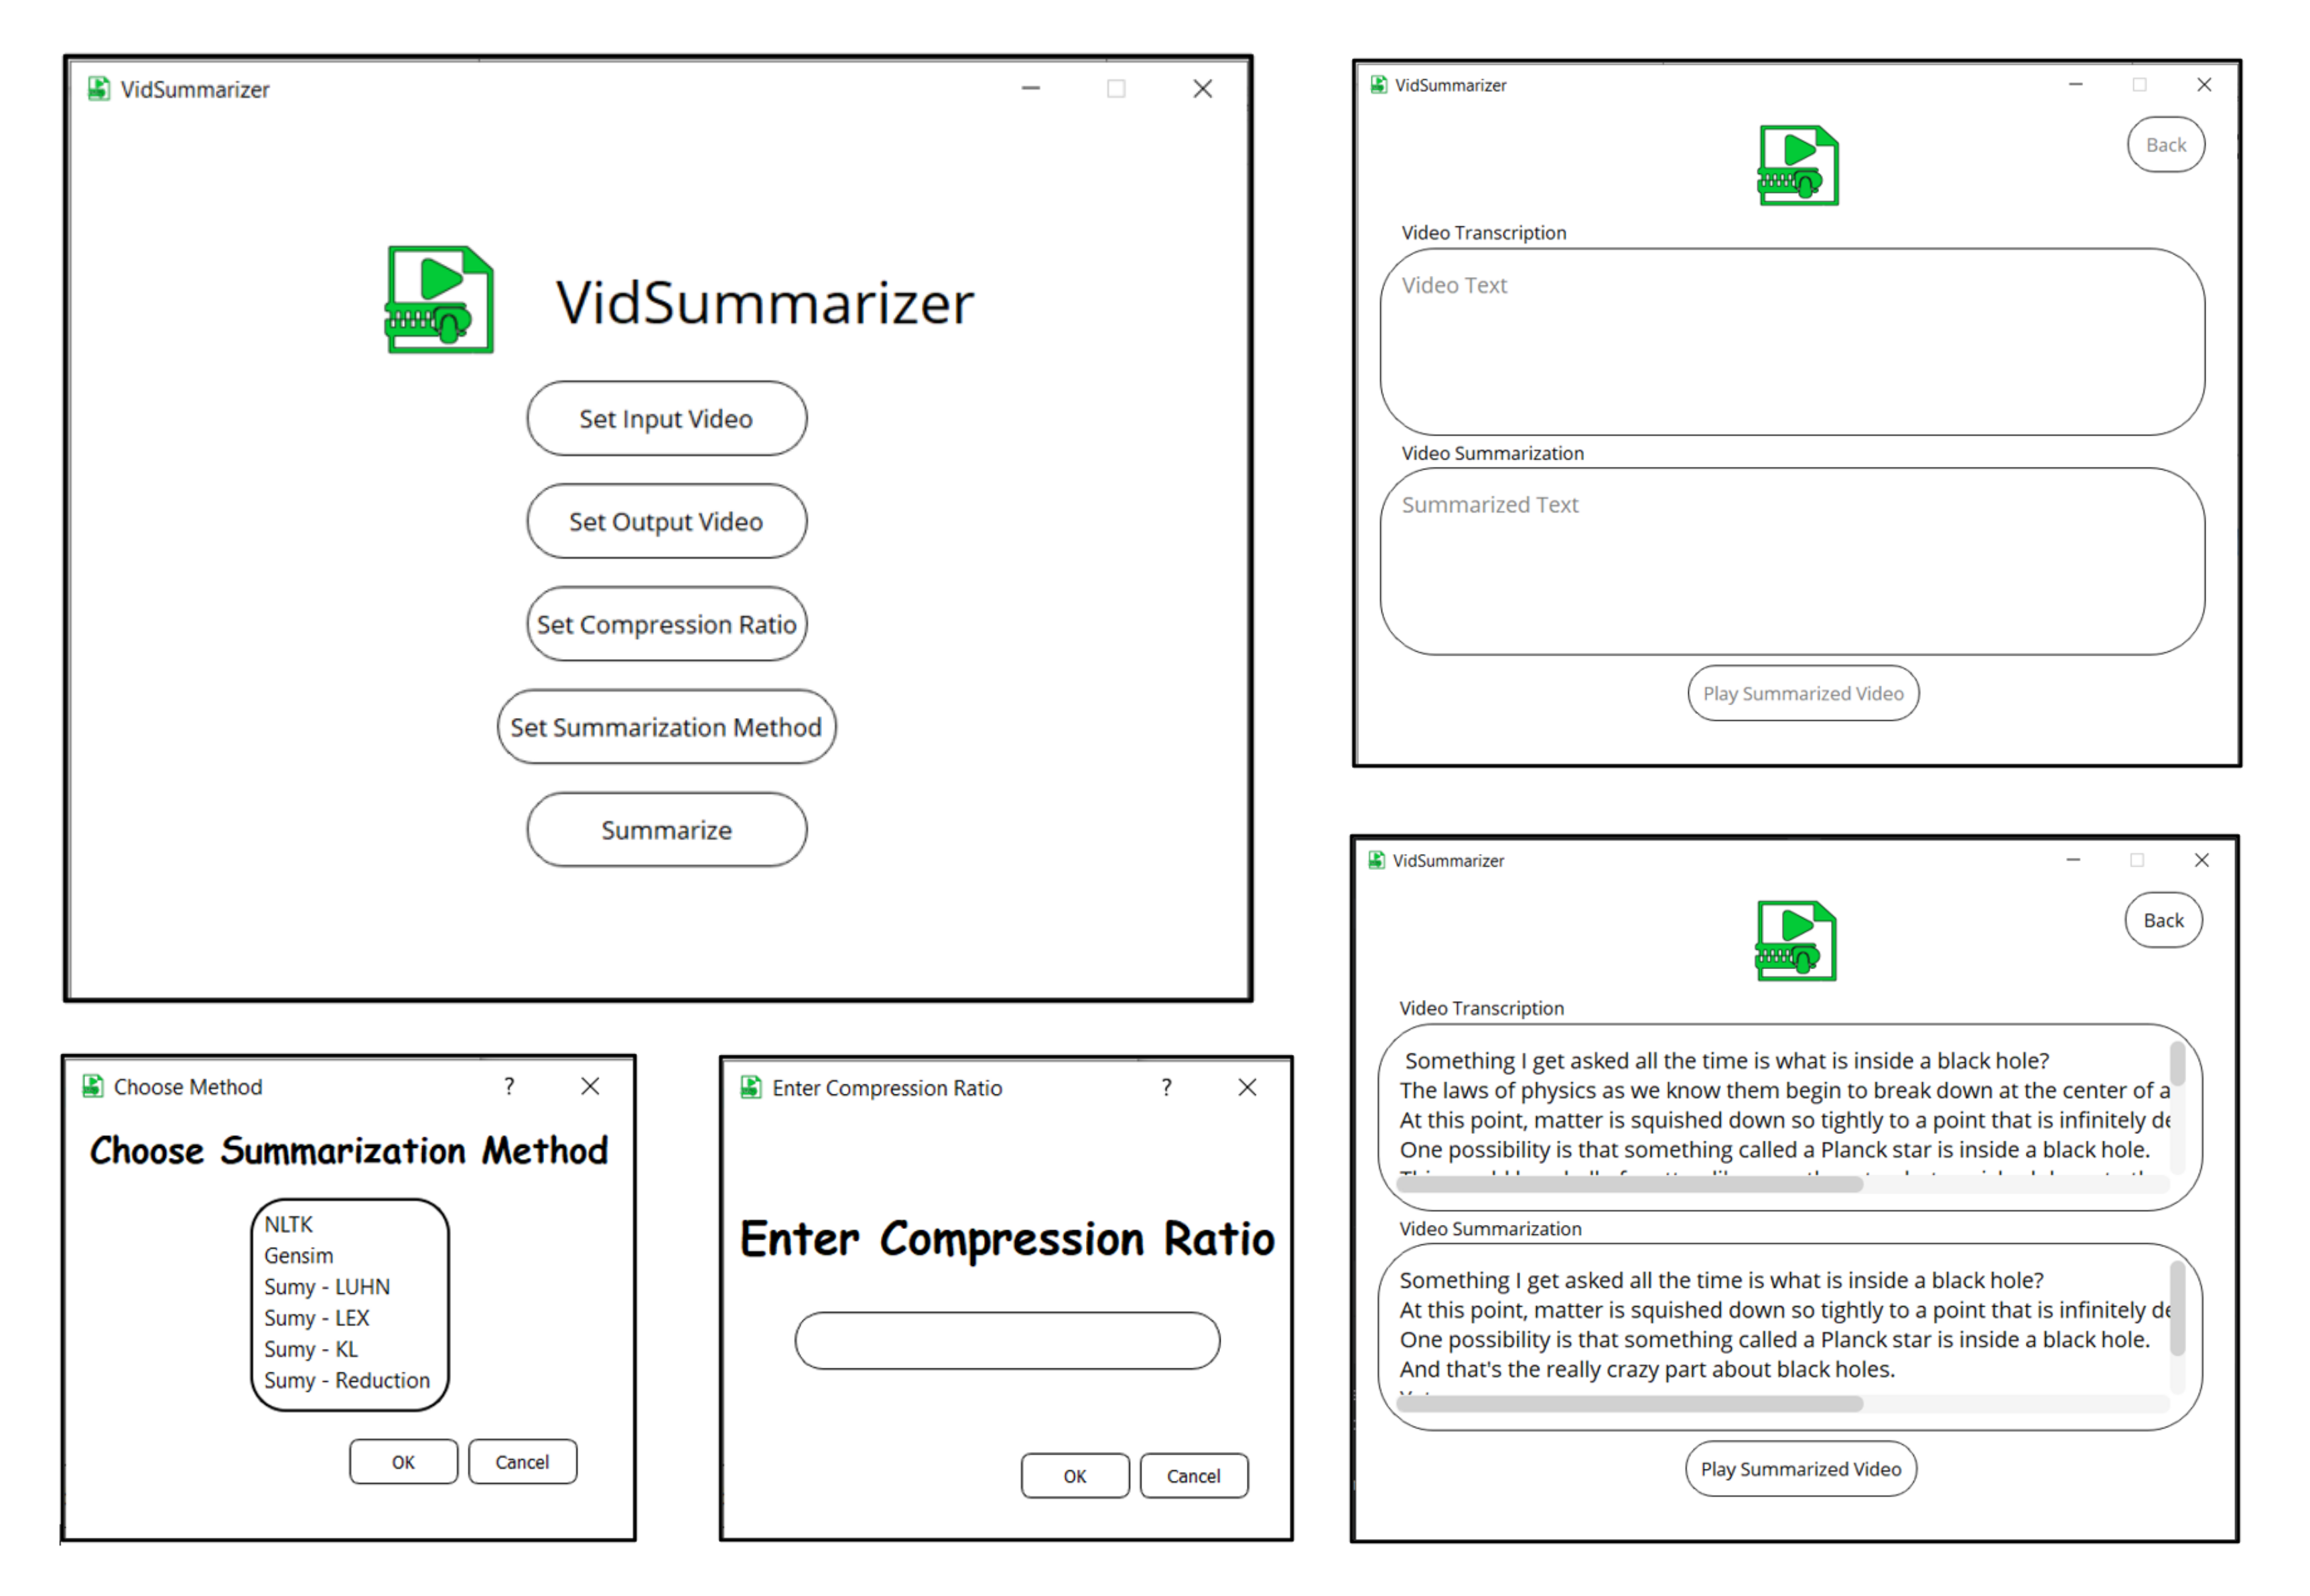
\includegraphics[width=9cm, height=10cm, keepaspectratio]{GUI.png}
    \caption{Application GUI}
    \label{application_gui}
\end{figure} 

\section{Tools Used}
\label{tools_used}
In the development of our video summarization application, a versatile array of tools was carefully selected to cover various aspects of the project, ranging from natural language processing to version control. Each tool played a unique role in shaping the application's functionality and overall success.

\begin{itemize}
    \item \textbf{Python:} A high-level programming language that served as the backbone of our implementation. Known for its readability and versatility, Python provided an environment conducive to rapid development, fostering efficient coding practices and facilitating seamless integration with a diverse set of libraries.

    \item \textbf{Gensim:} A robust natural language processing library for Python. Gensim played a pivotal role in implementing the TextRank Summarizer algorithm, allowing us to extract key information from textual content and contributing to the overall summarization capabilities of our application.

    \item \textbf{Sumy:} A Python library empowering our application with a range of summarization techniques, including KL-Sum, LexRank, Luhn, and Naive Reduction. Its modular architecture provided flexibility, enabling us to experiment with and integrate various summarization algorithms into our system.

    \item \textbf{json:} The json library in Python facilitated the parsing of Whisper responses, integral to our Speech-to-Text functionality. By converting responses into a structured JSON format, this tool enhanced data interchange and interaction between the speech-to-text module and the core application.

    \item \textbf{pyqt5:} PyQt5, a Python binding for the Qt framework, was instrumental in crafting our Graphical User Interface (GUI). Renowned for its simplicity and rich widget set, PyQt5 allowed us to design an intuitive and visually appealing interface, ensuring an engaging user experience.

    \item \textbf{nltk:} The Natural Language Toolkit (nltk) in Python facilitated word and sentence tokenization. Its comprehensive set of tools for natural language processing enriched the algorithmic components of our application, enhancing text analysis capabilities.

    \item \textbf{whisper:} Whisper, a Speech-to-Text tool, played a pivotal role in transcribing audio content extracted from videos. By converting spoken words into text, Whisper provided accurate and reliable data for further analysis and incorporation into the summarization process.

    \item \textbf{pydub:} Pydub, a Python library for audio processing, streamlined the extraction of audio from video content. Its functionalities, such as changing frame rates and sample widths, allowed us to handle audio data effectively and seamlessly integrate auditory content into the summarization process.

    \item \textbf{moviepy:} Moviepy, a Python library for video editing, proved indispensable in the creation and splitting of video content. Its capabilities enhanced our ability to manipulate video data efficiently, aligning with our goal of providing a comprehensive video summarization experience.

    \item \textbf{PIP (Python Package Installer):} PIP, short for Python Package Installer, simplified the installation of external Python packages. Its straightforward command-line interface and package management capabilities ensured a smooth and efficient process for incorporating dependencies into our development environment.

    \item \textbf{Git:} Git, a distributed version control system, played a vital role in collaborative development. By tracking changes, managing versions, and facilitating seamless collaboration among team members, Git ensured the integrity and stability of our codebase throughout the development lifecycle.
\end{itemize}
The meticulous selection and integration of these tools into our development environment contributed to the successful implementation of a feature-rich video summarization application. This aligns with our objectives of user-friendliness, functionality, and algorithmic diversity.

\section{Comparison with State-of-Art Methodologies}
\label{Comparison with State-of-Art Methodologies}
We have demonstrated the application's versatility by implementing multiple summarization algorithms, including but not limited to, the Pure NLTK Method, Gensim TextRank, and the advanced LexRank Method, each chosen for its unique ability to distill essential information from extensive video transcripts. Our approach aligns with advanced methodologies, as seen in \cite{ref9}, and addresses the personalization aspects of summarization akin to the contributions in \cite{ref7}. The efficiency of our system echoes the data processing advancements presented in \cite{ref6} and the innovative fast-forwarding mechanisms of \cite{ref10}.

Our application stands out by offering a user-friendly interface, integrating state-of-the-art algorithms that ensure both accuracy and efficiency. The results garnered from our experiments indicate that our approach not only holds its ground theoretically but also excels in practical applications. We anticipate that our contributions will significantly benefit domains requiring rapid and precise video analysis, providing a foundation for future advancements in the field.

\section{Conclusion}
\label{conclusion}
This study represents a significant stride in the field of video summarization, harnessing the capabilities of natural language processing to extract the essence of video content effectively. Our comprehensive exploration of machine learning, deep learning, and NLP-based techniques has culminated in the creation of a sophisticated application that epitomizes the cutting-edge of extractive summarization.

Through the implementation of multiple summarization algorithms, our application has exhibited remarkable versatility and robustness. Methods such as the Pure NLTK Method, Gensim TextRank, and the advanced LexRank Method have each played a pivotal role in refining the summarization process, ensuring that the most salient information is captured and presented in a condensed format.

The practicality of our application is evidenced by its user-friendly interface, which democratizes the use of advanced summarization techniques, making them accessible to a broader audience. The efficacy of the system has been validated through rigorous testing, showcasing not only theoretical soundness but also superior performance in real-world scenarios.

The implications of our work are vast and far-reaching, promising to enhance the efficiency with which video content is processed and understood. By offering rapid and precise analysis, our application lays the groundwork for significant improvements in areas such as media, education, and content curation.

Looking forward, we aim to expand the boundaries of our application even further. Future enhancements will focus on personalizing the summarization experience and incorporating the ability to process videos in real-time. These developments are anticipated to elevate the standard for video summarization technologies, fostering greater efficiency and engagement.

In closing, our research contributes a meaningful advancement to the video summarization toolkit, one that stands to reshape the landscape of video content analysis and utilization.



\section*{Author contributions}
All authors contributed equally to this paper, where all authors read and approved the work in this paper.



\bibliographystyle{plain}
\bibliography{ref}

\EOD
\end{document}
